\section{Systematics and expected sensitivity}
(outline by David)

\subsection{Systematics: unchanged}What is the same as Run 1-2-3 analysis: few sentences + reference past note.
\subsection{Systematics: What's new}
\subsubsection{GENIE FSI bug-fix} A few validation plots, e.g. Chris' validation work of GENIE weights.
\subsubsection{EXT smoothing} (Alex)
\subsubsection{DetVar systematics} Are we assuming Run123 detvars for Run 1-5? Probably true for first sensitivites. \\
Include a table which lists MC stats available on DetVar samples.
\subsubsection{Signal model systematics}

\subsection{systematics summary}

The total systematics error budget is shown in the table of Fig.~\ref{fig:systematicsbudget}.

\begin{center}
\begin{figure}[h]
    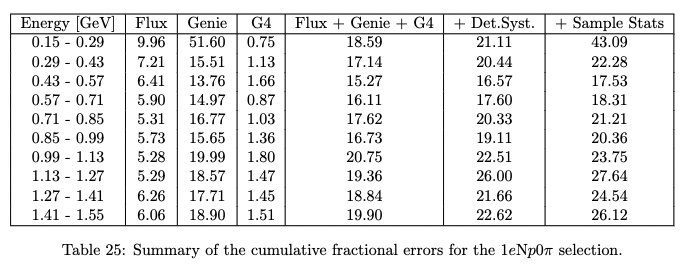
\includegraphics[width=1.00\textwidth]{technote/SystematicsSensitivity/Figures/systematicsbudget.png}
    \caption{Enu spectrum before/after constraint.}
    \label{fig:systematicsbudget}
\end{figure}
\end{center}

\newpage
\subsection{Constraints}
Describe briefly, refer to older analysis.

Show spectrum of nues before and after constraint. See Fig.~\ref{fig:constraint}.

\begin{center}
\begin{figure}[h]
    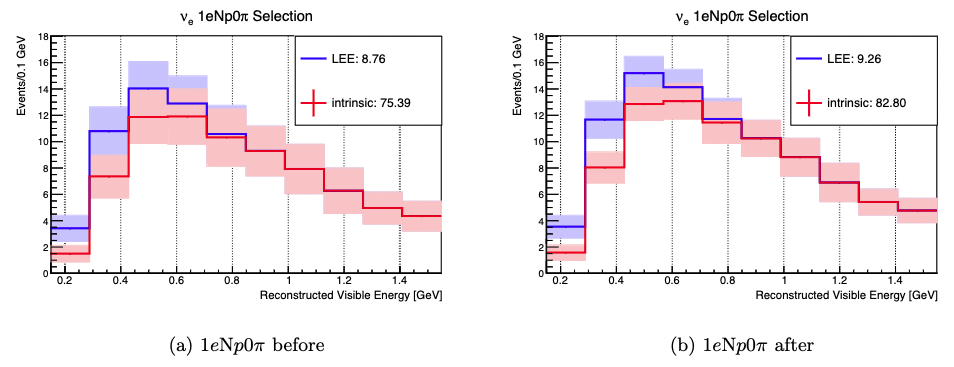
\includegraphics[width=1.00\textwidth]{technote/SystematicsSensitivity/Figures/constraint.png}
    \caption{Neutrino energy spectrum before/after constraint.}
    \label{fig:constraint}
\end{figure}
\end{center}

Show quantitative predicted events and uncertainty (including reduction in uncertainty) before/after constraint. See Table of Fig.~\ref{fig:constrainttable}.

\begin{center}
\begin{figure}
    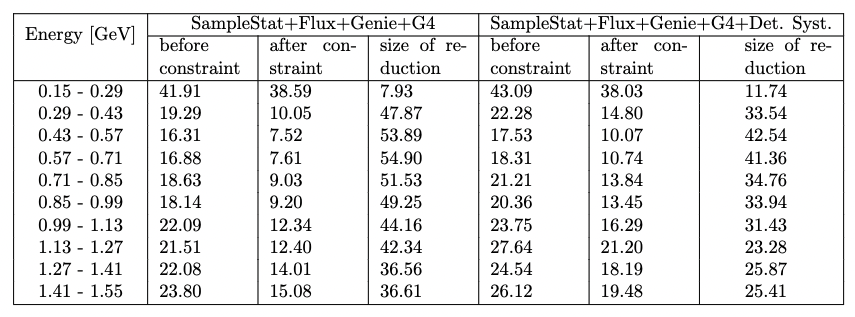
\includegraphics[width=1.00\textwidth]{technote/SystematicsSensitivity/Figures/constrainttable.png}
    \caption{Impact of constraint.}
    \label{fig:constraint} 
\end{figure}
\end{center}

Potentially think of new ideas here

\newpage
\subsection{Sensitivity}
\label{sec:sensitivity}

\subsubsection{Simple Hypothesis Test}

Distribution of test statistic for backgronud-only and signal models, with extracted median sensitivity. See. Fig.~\ref{fig:simplehypothesis}.

\begin{center}
\begin{figure}[h]
    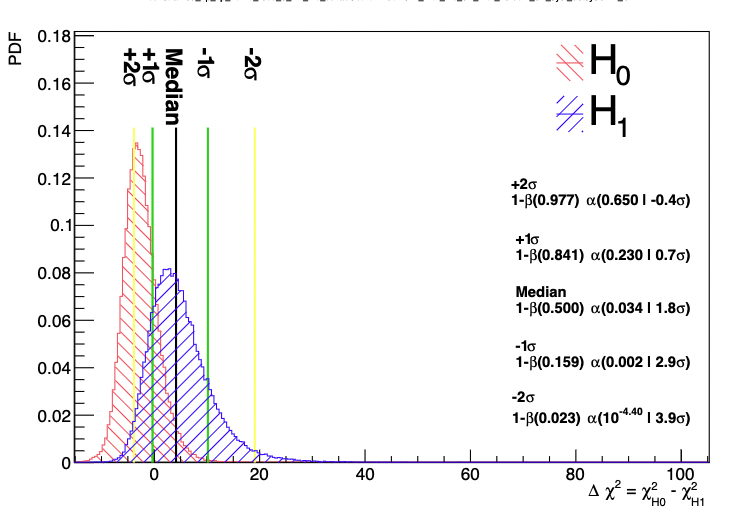
\includegraphics[width=1.00\textwidth]{technote/SystematicsSensitivity/Figures/simplehypothesis.png}
    \caption{Impact of constraint.}
    \label{fig:simplehypothesis} 
\end{figure}
\end{center}

Fig.~\ref{fig:simplehypothesisresults} shows the expected sensitivity for the simple hypothesis test.

\begin{center}
\begin{figure}[h]
    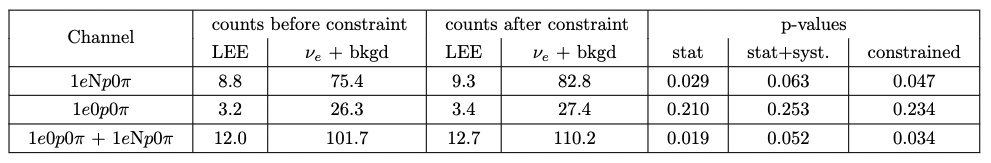
\includegraphics[width=1.00\textwidth]{technote/SystematicsSensitivity/Figures/simplehypothesisresults.png}
    \caption{Impact of constraint.}
    \label{fig:simplehypothesisresults} 
\end{figure}
\end{center}

\newpage
\subsubsection{Signal strength fit}

The signal strength sensitivity results are shown in Fig.~\ref{fig:signalstrengthsensitivity}.
\begin{center}
\begin{figure}[h]
    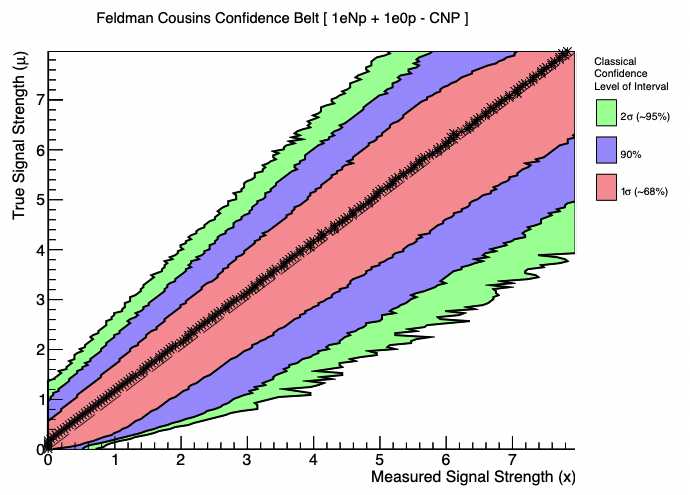
\includegraphics[width=1.00\textwidth]{technote/SystematicsSensitivity/Figures/signalstrengthsensitivity.png}
    \caption{Impact of constraint.}
    \label{fig:signalstrengthsensitivity} 
\end{figure}
\end{center}

\newpage
\subsubsection{Validation of sensitivity vs. SBNFit benchmark}
